\documentclass[letterpaper,twocolumn,openany,nodeprecatedcode]{dndbook}
\usepackage[english]{babel}
\usepackage[utf8]{inputenc}
\usepackage[singlelinecheck=false]{caption}
\usepackage{lipsum}
\usepackage{listings}
\usepackage{shortvrb}
\usepackage{eso-pic}
\usepackage{tikzpagenodes}
\usepackage{multicol}
\usepackage{float}
\usepackage{graphicx}

\captionsetup[table]{labelformat=empty,font={sf,sc,bf,},skip=0pt}

\MakeShortVerb{|}

\lstset{%
  basicstyle=\ttfamily,
  language=[LaTeX]{TeX},
  breaklines=true,
}
%Colocar imagem no fundo
\newcommand{\TitleBackground}{%
  \begin{tikzpicture}[remember picture,overlay]
    \node at (current page.center) {
      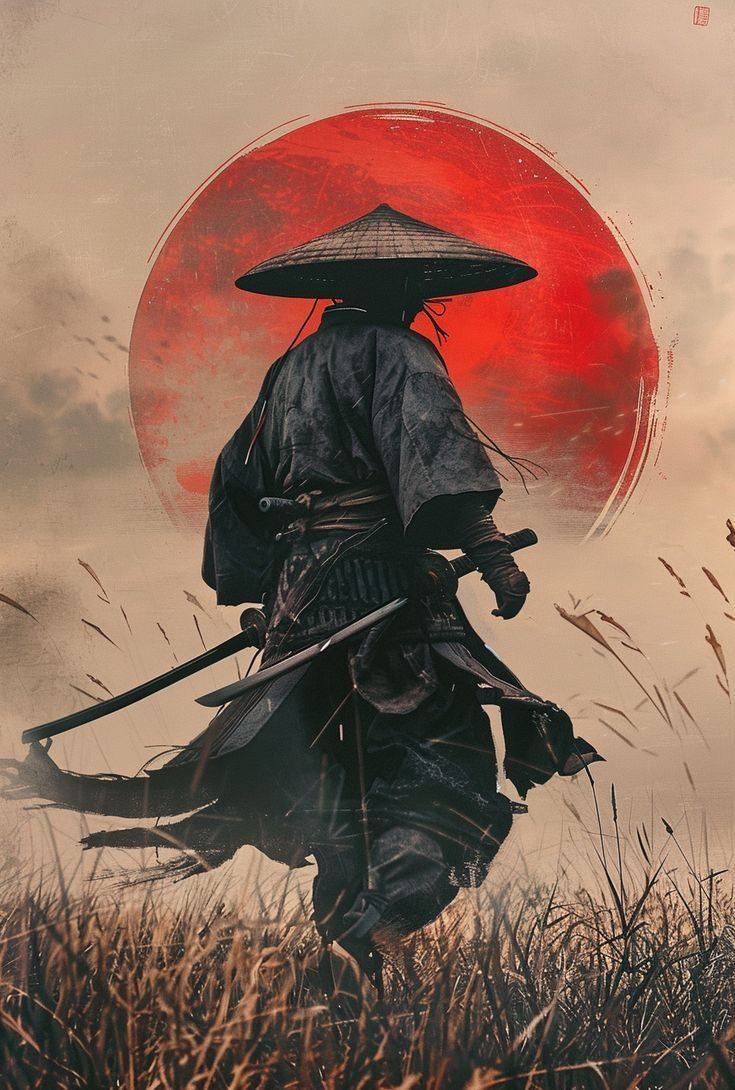
\includegraphics[width=\paperwidth,height=\paperheight]{img/Samurai_img.jpeg}};
  \end{tikzpicture}
}

\begin{document}

\frontmatter

\begin{titlepage}
    %imagem de fundo
    \TitleBackground
    
    %Título
    \vspace*{1cm}
    \begin{center}
        {\Huge\bfseries The Samurai\par}
        \vspace{0.5cm}
        {\large Adapt to the flow of combat with this homebrew martial class\par}
    \end{center}
\end{titlepage}

\clearpage
\tableofcontents


\mainmatter

\section{The Samurai}

\DndDropCapLine{S}{tanding alone beneath a barren ladscape, a human faces down a legion of Orc 
    soldiers with a single blade in hand, his liege, a 10-year old princeling, 
    quivering behind him.}
\\ 
Hidden in the shadows of a mansion's ceilling, an elevn spy watches a gathering
of lords having a wat council, taking notes on their battle strategies.
He keeps his set of bizarre equipment close to him, ready to scape at a moment's 
notice.  
\vspace{\baselineskip}

\noindent Talismans in hand, a dragonborn priest summons spirit animals that hold down a 
demon-possessed civilian. A blaze of fire suddenly silences de demon's cries, as 
he finally draws out the creature that's been terrorizing the village.
\vspace{\baselineskip}

\noindent Beholden by an oath no dissimilar to a knight, Samurai pledge their services to 
a single individual, devoting their life to their cause. No matter the vast 
diferrences in treir chosen lord, Samurai undergo a specialized training that 
focus on a certain set of skills, skills that are sometimes as varied as the lord 
they choose to serve. Whether skilled warriors who master the art of the blade, 
subterfuge experts trained in gathering intel and assassination, or learned 
arcanists who channel divine energy through esorteric implements, Samurai are 
renowned and respected by their unering dedication to their craft.

\subsection{A loyal Vassal}
Samurai more often than not, enter into the service of a lord when they begin their 
training. Perhabs they're apprenticed indo the lord of the land, or a family member 
has taken them up for training, whichever the case, Samurai spend their early training 
days working closely with their liege.
\vspace{\baselineskip}

\noindent Their oath is bound by honor. Thus, they perform their services until their death and 
nothing would bring a Samurai greater shame than being dishonorably dismissed. Their 
master's death is no reason for a Samurai's duty to ente either.
Most Samurai pass on their services to their master's family, or to someone that their 
ma+ster deems close. A few of them become lords themselves and even fewer settel down 
and retire.

\begin{DndComment}{Multiclassing}
    You need a Strength and Dexterity of 13 to multiclas in and out of this class.


    \textbf{Proficiencies}: Light armor, Simple Weapons, Martial Weapons, Calligrapher's Tools, Smith's Tools.
\end{DndComment}

\subsection{Distant Wanderers}
In an event that a Samurai becomes without a lord, they might prefer to continue their 
duties on their own, drifting from one place to another, only stopping at an area to 
replenish their supplies or take a brief respite.
\vspace{\baselineskip}

\noindent These Samurai are referred to as \textbf{Ronin}, someone who finds the way without 
belonging to one place. They can often be seen living and traveling amongst the commonfolk,
assisting them in times of trouble and defending their vilages from bandits and raiders.
\vspace{\baselineskip}

\noindent These Samurai live a simpler life, but their hearts remain ready for the call of adventure.

\begin{DndReadAloud}
    \begin{figure}[H]
        \centering
        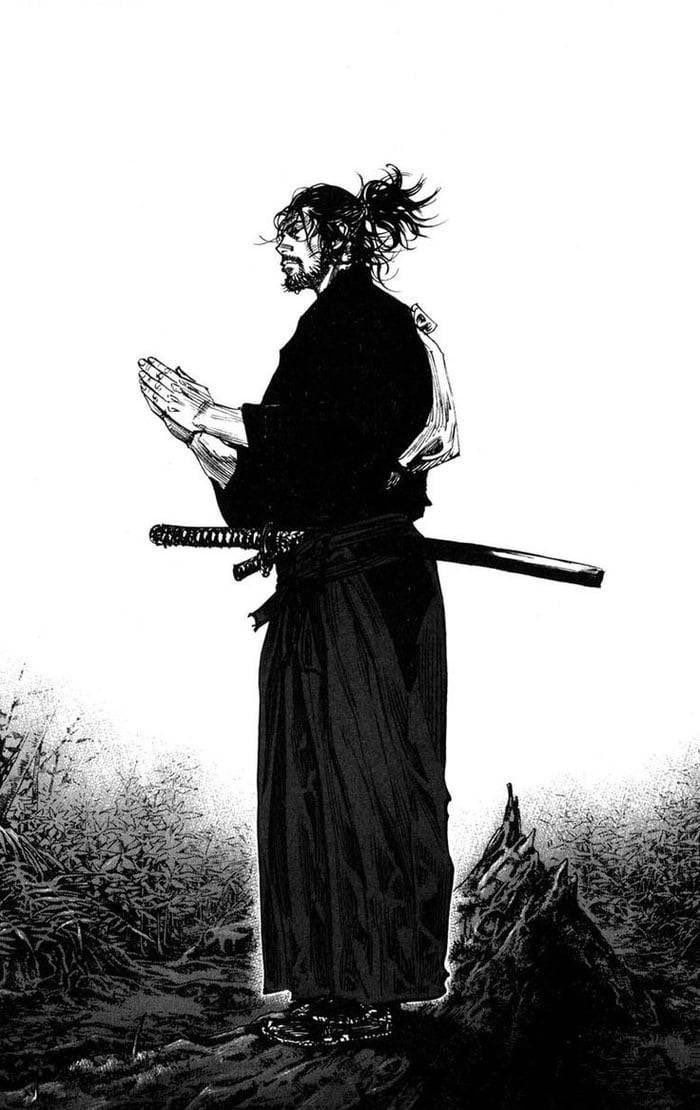
\includegraphics[width=\columnwidth]{img/Musashi_Myamoto.jpeg}
    \end{figure}
\end{DndReadAloud}
\newpage
\section{Samurai Weapons}
Those who follow the code of Samurai, come from all walks of life, but its true origins lie in
an archaic culture tha existed long ago. If you wish to create a Samurai that comes from that
path, here are some of the names and descriptions of the weapons they choose to wield.
Whatever names you use for a Samurai Weapon, you can use the game statics provided for the weapon
on the weapons page of the Player's Handbook.

\begin{DndTable}[header= Samurai Weapons]{XX}
    \textbf{Name} & \textbf{Description} \\
    Bo (quaterstaff) & A staff made from unfinished hard wood or a flexible wood, such as red or white oak \\
    Kama (Sickle) & A farming implement similar to a sickle, used for reaping crops and also employed as weapon \\
    Kanabo (Warhammer) & A spiked or studded two-handed war club \\
    Katana (Longsword) & A curved, single-edged blade with a circular or squared guard and long grip to accommodate to hands. The trademark of the Samurai \\
    Kusari-fundo (Flail) &  A hand-held weapon consisting of a length of chain (kusari) with a weight (fundo) attached to each end of the chain \\
    Naginata (Glave) & A pole weapon that consists of a wooden or metal pole with a curved, single-edged blade on the end \\
    Odachi (Greatsword) & A traditionally made katana with a longer and heavier blade \\
    Otsuchi (Maul) & A large wooden mallet \\
    Tanto (Dagger) & A dagger that Samurai use as a last resort or self-defense \\
    Wakizashi (Shortsword) & A smaller version of the katana. Often seen as a pair together with the katana called Daisho (Big and Small) \\
    Yari (Spear) & A form of straight headed spear. Yari often have varied points of blade attached to its tip \\
    Yumi (Longbow) & An assimetrical bow that's exceptionally tall\\
\end{DndTable}

\begin{DndComment}{Mastery}
    Each Samurai weapon can use the the mastery of the correspondent classical weapon of the Player's Handbook
\end{DndComment}

\begin{DndReadAloud}
    \begin{figure}[H]
            \centering
            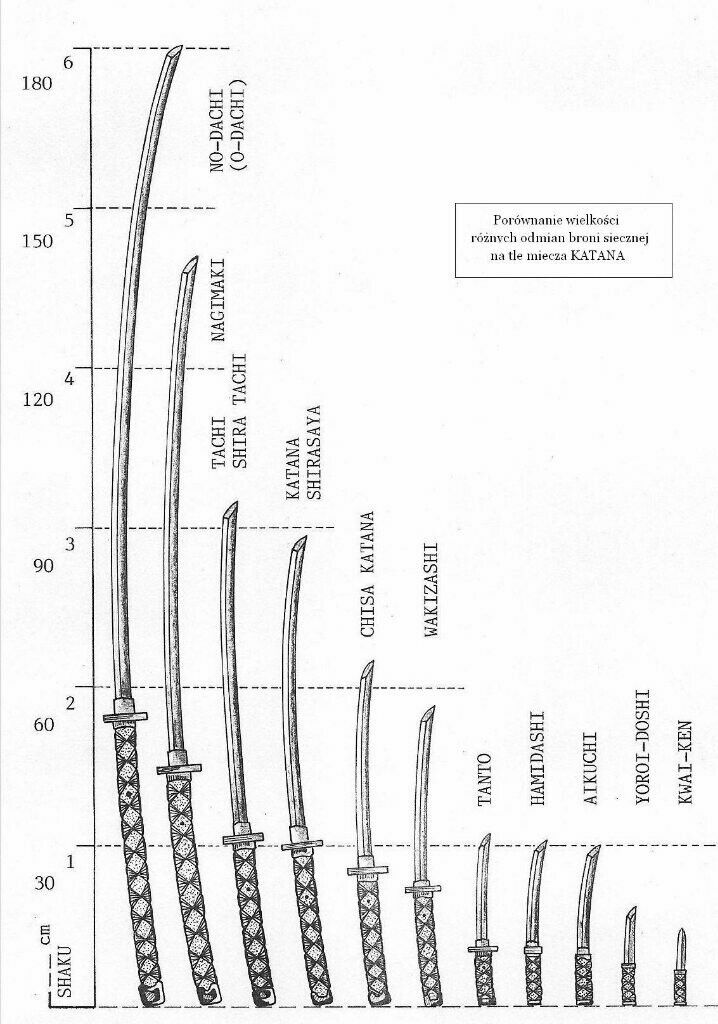
\includegraphics[width=\columnwidth]{img/swords.jpg}
    \end{figure}    
    \begin{figure}[H]
            \centering
            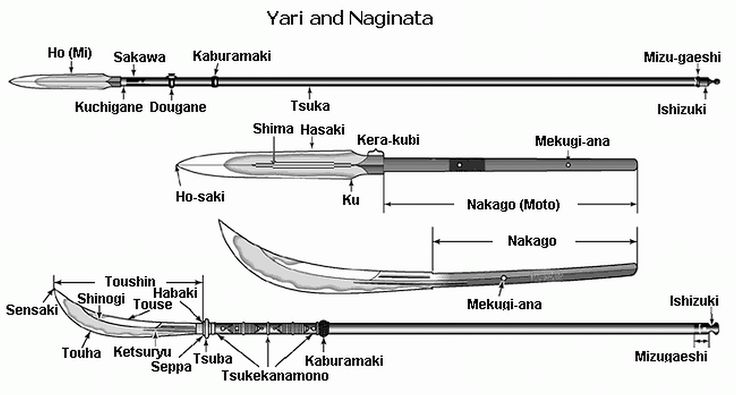
\includegraphics[width=\columnwidth]{img/Yari_and_naginata.jpg}
    \end{figure}    
\end{DndReadAloud}

\newpage

\section{Samurai}

\begin{tcolorbox}[
  enhanced,
  colback=white,
  colframe=black!85,
  boxrule=0.9pt,
  arc=2mm,
  drop shadow,
  left=6pt,
  right=6pt,
  top=6pt,
  bottom=6pt,
  width=\textwidth
]
\begin{DndTable}[header= The Samurai]{ccXcccc}
    \textbf{Level} & \textbf{PB} & \textbf{Features} & \textbf{Heaven} & \textbf{Earth} & \textbf{Man} & \textbf{Mastery}\\
    1st & +2 & Stance, First step, Mastery & 1d4 & 10ft. & +2 & 2\\
    2nd & +2 & Elegant Courtier, Fighting Style & 1d4 & 10ft. & +2 & 2\\
    3rt & +2 & Samurai Discipline Feature & 1d4 & 10ft. & +2 & 2\\
    4th & +2 & Ability Score Improvement, Martial Versatility & 1d4 & 10ft. & +2 & 3\\
    5th & +3 & Extra Attack, Precise Strike & 1d6 & 10ft. & +3 & 3\\
    6th & +3 & First Step Improvement, Ascended Stance & 1d6 & 15ft. & +3 & 3\\
    7th & +3 &  & 1d6 & 15ft. & +3 & 3\\
    8th & +3 &  & 1d6 & 15ft. & +3 & 3\\
    9th & +4 &  & 1d6 & 15ft. & +3 & 3\\
    10th & +4 &  & 1d6 & 15ft. & +3 & 4\\
    11th & +4 &  & 1d8 & 15ft. & +4 & 4\\
    12th & +4 &  & 1d8 & 15ft. & +4 & 4\\
    13th & +5 &  & 1d8 & 20ft. & +4 & 4\\
    14th & +5 &  & 1d8 & 20ft. & +4 & 4\\
    15th & +5 &  & 1d8 & 20ft. & +4 & 4\\
    16th & +5 &  & 1d8 & 20ft. & +4 & 4\\
    17th & +6 &  & 1d10 & 20ft. & +5 & 4\\
    18th & +6 &  & 1d10 & 20ft. & +5 & 4\\
    19th & +6 &  & 1d10 & 20ft. & +5 & 4\\
    20th & +6 &  & 1d10 & 30ft. & +5 & 4\\
\end{DndTable}
\end{tcolorbox}

\begin{figure}[H]
    \centering
    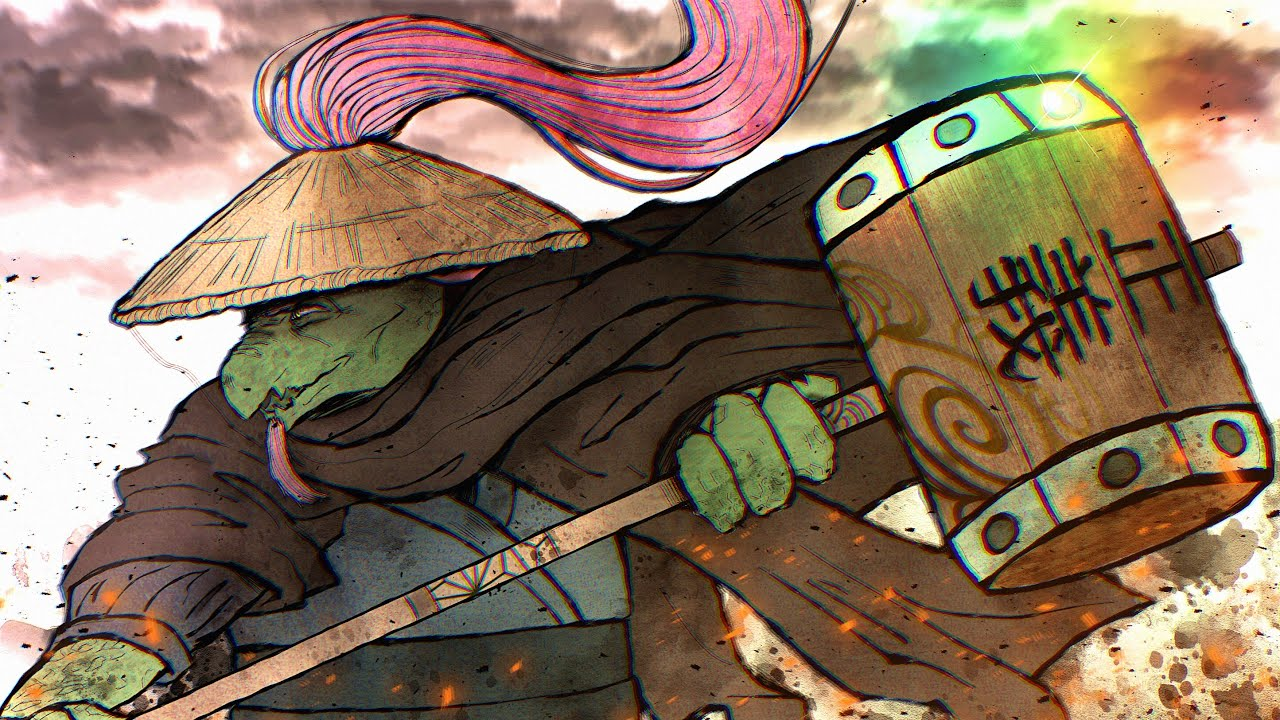
\includegraphics[width=\textwidth]{img/otsushi_of_justice.jpg}
    \Caption{The Hammer of Justice}
\end{figure}

\newpage
\clearpage
\newpage
\subsection{Class Features}
As a Samurai, you gain the following class features
\subsubsection{Hit Points}
\textbf{Hit Dice:} 1d10 per Samurai Level\\
\textbf{Hit Points at 1st Level:} 10 + your Constitution modifier\\
\textbf{Hit Points at higher levels:} 1d10(or 6) + your Constitution modifier per Samurai level after 1st\\

\subsubsection{Proficiencies}
\textbf{Armor:} Light and medium armors\\
\textbf{Weapons:} Simple and martial weapons\\
\textbf{Tools:} Calligrapher's and Smith's tools\\
\textbf{Saving Throws:} Strength and Constitution\\
\textbf{Skills:} Choose two from Athletics, Acrobatics, Insight, Intimidation, Persuasion, Perception\\

\subsubsection{Equipment}
You start with the following equipment, in addition to the equipment granted by your background:
\begin{itemize}
    \item (a) scale mail or (b) leather armor
    \item (a) a longsword and a shortsword or (b) two martial weapons
    \item (a) a diplomat's pack or (b) a explorer's pack
    \item (a) calligrapher tools or (b) smith's toolsr
    \item longbow and 20 arrows
\end{itemize}

\subsubsection{Stance}
Your unique training gives you access to stances that let you adapt to any situation. On your turn, before
you attack, you can enter a stance as a bonus action.

\noindent While in a stance, you gain benefits based on the stance of your choice, provided that you aren't yousing a 
shield.
\vspace{\baselineskip}

\paragraph{Heaven}
The heavenly stance, high and mighty, deliver intense and powerfull strikes, designed to cut 
down even strongest foes.

\begin{itemize}
    \item Your weapon damage rolls deal an extra 1d4 damage, which you roll twice when you crit. This damage
    die increases by one size - e.g 1d4 to 1d6 - when you use a two handed melee weapon or a longbow to make
    an attack.
\end{itemize}
\vspace{\baselineskip}

\paragraph{Earth}
The earth stance, sturdy as a rock, maintains a steady and balanced footing, letting you move
swiftly across the batlefield.

\begin{itemize}
    \item Your speed is increased by 10ft.
    \item When you make a melee attack against a creature and hit, you don't provoke opportunity attacks from 
    that creature for the rest of the turn. %edição feita por Otávio
\end{itemize}
\vspace{\baselineskip}

\paragraph{Man}
The stance of Man, lowly and cautious, favor defensive posturs that let you evade or mitigate the
damage you receive.

\begin{itemize}
    \item Whenever you make a Dexterity saving throw while in this stance, you can roll a d4 and add the number
    rolled to the saving throw. 
    \item You gain a +2 bonus to AC.
\end{itemize}

\noindent Your stance lasts for one minute, ultil you enter a diferent stance, or until you are incapacitated. You can also
end your stance on your turn as a bonus action.

\noindent The bonuses you gain from your stances increase when reach certain Samurai levels, as show in the Samurai Table.

\subsubsection{First Step}
At first level, your first step is quicker than most, thanks in part to your martial acuity. You gain a bonus to
your initiative rolls equal to your proficiency bonus.
\vspace{\baselineskip}

\noindent Starting at 6th level, if you are surprised at the beginning of combat and aren't incapacitated, you can act 
normally on your first turn, but only if you enter a stance before doing anything else on that turn.
\vspace{\baselineskip}

\noindent At 13th level, your unmached speed and discipline gives you advantage on initiative rolls.

\subsubsection{Weapon Mastery}
Your training with Samurai weapons allows you to use mastery properties with two types of weapons of your choice, 
such as kamas or odachis. Whenever you finish a long rest, you can practice and replace one of these weapon choices.

\noindent As you reach certain Samurai levels, you gain additional weapon choices, as shown in the Samurai table.

\newpage
\subsubsection{Elegant Courtier}
Starting at 2nd level, your discipline and attention to detail allow you to excel in social situations. Whenever you 
make a Charisma(Persuasion) check, you gain a bonus to the check equal to your wisdom modifier.
\vspace{\baselineskip}

\noindent At 11th level, your self-control also causes you to gain proficiency in wisdom saving throws. If you already have this
proficiency, you instead gain proficiency in Intelligence or Charisma saving throws (your choice). 

\subsubsection{Fighting Style}
At 2nd level, you adopt a particular style of fighting as your specialty. Choose one of the following options. You can't 
take a Fighting Style option more than once, even if you later get to choose again.
\vspace{\baselineskip}
\begin{itemize}
    \item \textbf{Archery:} You gain a +2 bonus to attack rolls you make with ranged weapons.
    \item \textbf{Blind Fighting:} You have blindsight with a range of 10 feet. Within that range, you can effectively see
    anything that isn't behind total cover, even if you are blinded or in darknes. Moreover, you can see an invisible creature
    within that range, unless the creature successfully hides from you.
    \item \textbf{Dueling:} When you are wielding a melee weapon in one hand and no other weapons, you gain a +2 bonus to damage
    rolls with that weapon.
    \item \textbf{Great Weapon Fighting:} When you roll a 1 or 2 on damage die for a attack made with a melee weapon that you are 
    wielding with two hands, you can reroll the die and must use the new roll, even if you rolled a 1 or 2. The weapon must have 
    the two-handed or versatile property for you to gain this benefit.
    \item \textbf{Throw Weapon Fighting:} You can drawn a weapon that has the throw property as part of the attack you make with 
    the weapon. In addition, when you hit with a ranged attack, you gain a +2 bonus to the damage roll.
    \item \textbf{Two-Weapon Fighting:} When you engage in two-weapon fighting, you can add your ability modifier to the damage of 
    the second attack.
\end{itemize}
\noindent At 10th level, you can choose an addition Fighting Style.

\subsubsection{Samurai Discipline}
At 3rt level you choose the type of School you specialize in. Your choice grant you features at 3rt leven and again at 9th, 15th and 20th level.

\subsubsection{Ability Score Improvement}
When you reach 4th level, and again at 8th, 12th and 16th level you can increase one ability score of your choice by 2, or you can choose 2 ability 
scores to increase by 1. As normal, you can't increase a ability score above 20 using this feature.

\subsubsection{Martial Versatility}
Whenever you reach a level in this class that grant you Ability Score Improvement feature, you can replace a fighting style you know with another
fighting style available to Samurai. This replace represents a shift of focus in your martial practice.

\subsection{Extra Attack}
Beginning at 5th level, you can attack twice, instead of once, whenever you take the attack action on your turn.

\subsection{Precise Strike}
Starting at 5tf level, you've become adept at turning your failures into advantage.
\vspace{\baselineskip}

\noindent When you miss a creature with a weapon attack, your next attack against that creature is made with advantage.

\subsubsection{Ascended Stance}
Beginning at 6th level, you can activate a stance's \textbf{Kai}. For 1 minute, this stance has additional benefits, along with the features it initially provides.
\vspace{\baselineskip}

\paragraph{Heaven Kai:} When you deal the additional damage of your Heaven stance, you can roll two dice instead of just one, adding both to the roll. If the target is incapacitated, prone or restrained, you deal maximum damage with both dice, instead of rolling them.
\vspace{\baselineskip}
\paragraph{Earth Kai:}
\vspace{\baselineskip}
\paragraph{Man Kai:}




\end{document}
